% book模板
% book模板.tex

\documentclass[12pt,UTF8]{ctexbook}

% 设置纸张信息。
\input{../../../common/page}

% 设置字体，并解决显示难检字问题。
\xeCJKsetup{AutoFallBack=true}
% 注意：ctexbook类已默认设置SimSun为CJKrmdefault
% 以下设置用于确保字体回退和扩展字体可用
% 仅设置扩展字体以避免与默认设置冲突
\setCJKfamilyfont{hei}{SimHei}
\setCJKfamilyfont{kai}{KaiTi}

% 目录 chapter 级别加点（.）。
\usepackage{titletoc}
\titlecontents{chapter}[0pt]{\vspace{3mm}\bf\addvspace{2pt}\filright}{\contentspush{\thecontentslabel\hspace{0.8em}}}{}{\titlerule*[8pt]{.}\contentspage}

% 支持目录点击跳转
\usepackage[colorlinks,linkcolor=blue,citecolor=blue,urlcolor=blue]{hyperref}

% 设置 part 和 chapter 标题格式。
\ctexset{
	part/name= {第,卷},
	part/number={\chinese{part}},
	chapter/name={第,篇},
	chapter/number={\arabic{chapter}}
}

% 图片相关设置。
\usepackage{graphicx}
\graphicspath{{Images/}}

% 设置署名格式。
\newenvironment{shuming}{\hfill\zihao{4}}

% 注脚每页重新编号，避免编号过大。
\usepackage[perpage]{footmisc}

% 设置古文原文格式。
\newenvironment{yuanwen}{\bfseries\zihao{4}}

% 设置段落间距
\setlength{\parskip}{0.8em plus 0.2em minus 0.1em}

% 列表格式支持，列表项向右偏移。
\usepackage{enumitem}

% 数学公式支持
\usepackage{amsmath}

\title{\heiti\zihao{0} 题目}
\author{WangFei}
\date{\today}

\begin{document}

\maketitle
\tableofcontents

\frontmatter
\chapter{前言、序言}

\mainmatter

\part{基础理论}
\label{part:basics}

\chapter{无线电入门}
\label{chap:intro}

\section{调制}

收音机是将调制过的音频信号解调、放大，最后通过扬声器等输出的设备。那么为什么不能直接接收未调制的音频信号呢？

音频信号的频率范围通常在 20 Hz 到 20 kHz 之间，属于低频信号。这样的低频信号如果直接通过天线发射，会遇到两个主要问题：

\begin{enumerate}[leftmargin=2cm]
	\item \textbf{天线效率极低}：天线的有效长度通常需要与信号波长的四分之一相当。对于 1 kHz 的音频信号，根据波长公式 $\lambda = c / f$，其中光速 $c \approx 3 \times 10^8$ m/s，可算出波长约为 300 公里，所需天线尺寸巨大，无法实际实现。
	\item \textbf{信道复用困难}：可用的音频频段非常窄，且拥挤不堪。如果不经调制直接发射，所有电台的信号都会混在一起，互相干扰，因为所有音频信号都挤在同一频段，接收端无法通过调谐来分离不同电台。
\end{enumerate}

因此，音频信号需要通过调制，将其"搭载"到高频载波上。高频载波就像一个"运输工具"，把音频信号"装载"上去，方便发射和传播。高频载波（例如几百 kHz 到几百 MHz）的波长短，天线尺寸小，且不同电台可使用不同载波频率，从而在空间中互不干扰地传播。

收音机接收到的电台信号通常有两种，调幅 AM 和调频 FM。波形图如下：

\begin{figure}[htbp]
	\centering
	%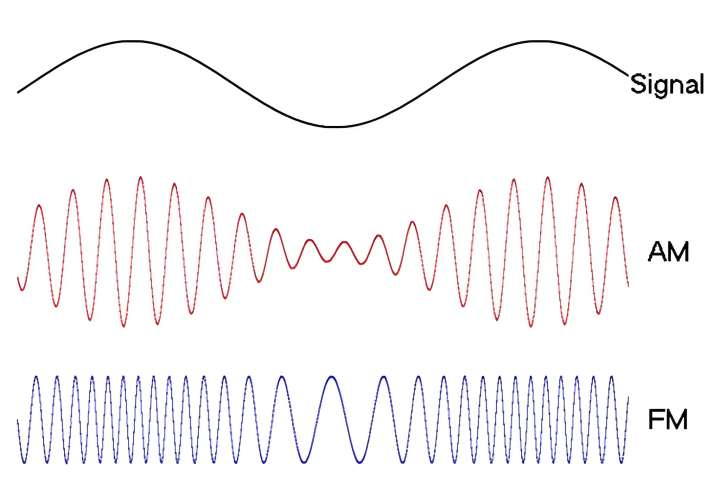
\includegraphics[width=0.7\linewidth]{am-fm-waveform.jpg}
	\caption{AM 与 FM 波形图}
	\label{fig:am-fm}
\end{figure}

从上图可以看出来：

\begin{itemize}[leftmargin=2cm]
	\item AM：载波的振幅随音频信号变化，但频率不变。
	\item FM：载波的频率随音频信号变化，但振幅不变。
\end{itemize}

以上过程称为调制，解调是其相反过程，会在后面进行说明。

\section{波段}

"波段"指的是无线电波中一段特定的频率范围。根据国际规定，调幅广播和调频广播分别使用以下频段：

\begin{itemize}[leftmargin=2cm]
	\item AM 波段：530 kHz -- 1600 kHz，属于中波波段。中波传播特性与超短波不同，可通过地波和天波传播，覆盖范围更广。
	\item FM 波段：87.5 MHz -- 108 MHz，属于超短波/甚高频波段。
\end{itemize}

明确了什么是调制以及电台信号所在的波段后，接下来我们看看收音机内部是如何将电波还原成声音的。


\part{矿石收音机}
\label{part:crystal-radio}

\chapter{矿石收音机基础}
\label{chap:crystal-radio-basics}

\section{矿石收音机总述}

这是最经典的入门电路，借用前辈书中的插图，最简单的电路和接线图如下：

\begin{figure}[htbp]
	\centering
	%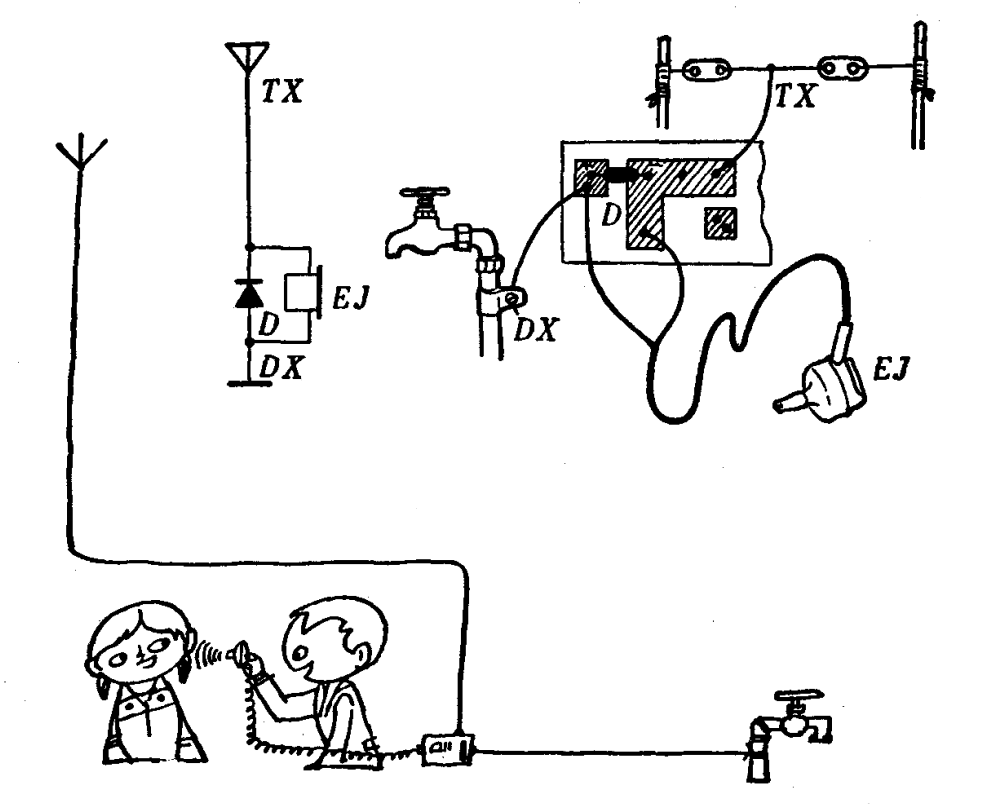
\includegraphics[width=0.7\linewidth]{simple_radio_circuit.png}
	\caption{矿石收音机电路图}
	\label{fig:crystal-radio-circuit}
\end{figure}

图片来源：朱蔼初编著的《看图学装收音机》

图中展示的是矿石收音机的典型结构，它由天线、晶体二极管、耳机、地线 4 个核心部件组成，本质上是一个无源接收装置。它利用半导体材料的整流特性接收无线电信号，不需要外接电源，完全依靠天线接收的无线电波能量工作。适用于接收 AM 电台的信号。

\section{各部件功能}

\subsection{1. 天线}

接收空间中传播的无线电波，这些电波会在天线中感应出微弱的高频交变电流。

在两个绝缘的竿子之间横拉一根电线即可，高度越高越好。在楼上，可用鱼竿挑出一根电线，离开墙体越远越好，谨防掉落。

\textbf{特别警示}：架设天线必须高度重视防雷，雷雨天气严禁使用，并应采取必要的避雷措施！

\subsection{2. 晶体二极管}

作为检波器，利用半导体的"单向导电性"，对天线接收到的高频信号进行检波（将调幅信号的高频载波去掉，提取音频信号）。

早期使用矿石检波器，这就是矿石收音机中"矿石"二字的来源。有活动矿石和固定矿石两种。活动矿石和固定矿石结构类似，核心就是矿石。常见有黄铁矿、方铅矿、红锌矿、自然铜等的金属矿石，结构如图。

\begin{figure}[htbp]
	\centering
	%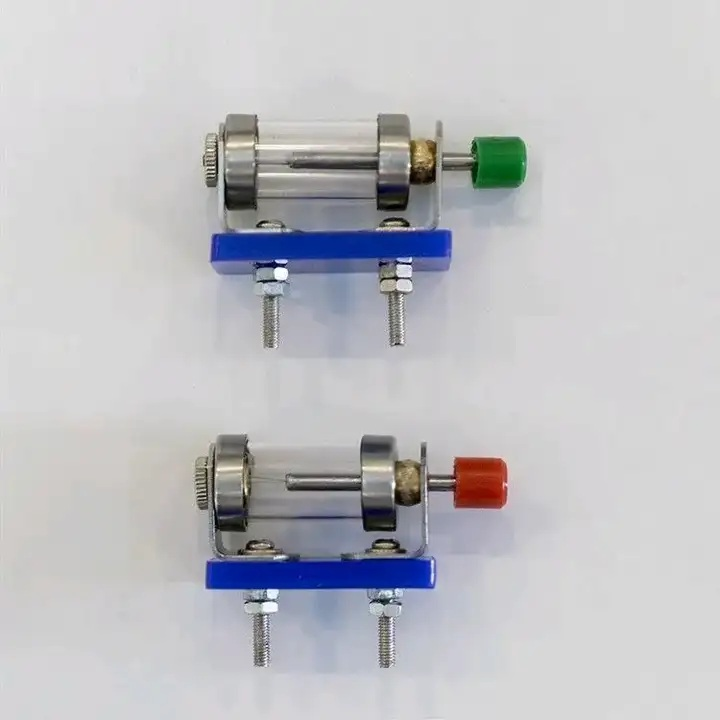
\includegraphics[width=0.7\linewidth]{mineral-detector.jpg}
	\caption{矿石检波器}
	\label{fig:mineral-detector}
\end{figure}

现在已无此必要，因为矿石价格不菲、调整麻烦且效果不理想。建议采用晶体二极管替代。型号可选 2AP9、1N60P 等，根据经验，1N60P 是个不错的选择。

\begin{figure}[htbp]
	\centering
	%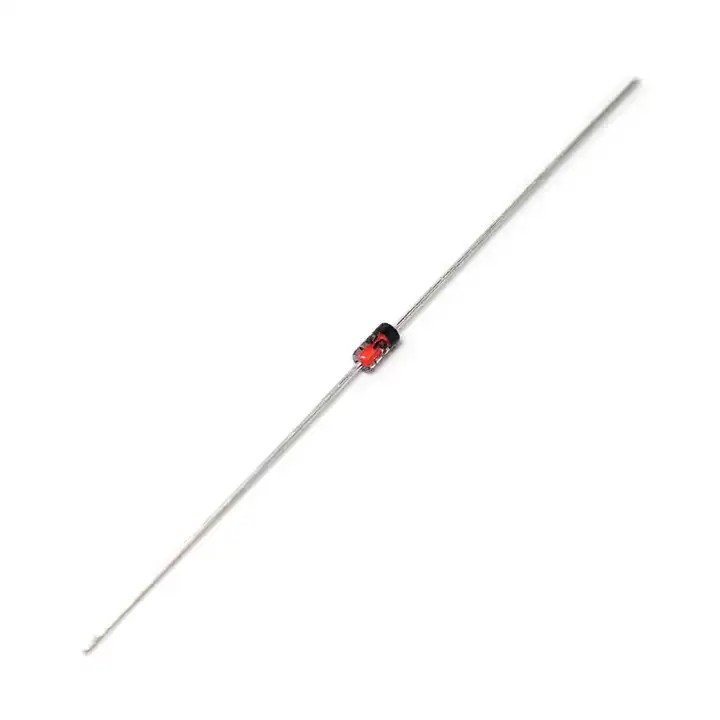
\includegraphics[width=0.7\linewidth]{1n60p.jpg}
	\caption{1N60P 二极管}
	\label{fig:1n60p}
\end{figure}

如果纯粹出于怀旧，完全可以采用矿石检波器，采购成品或自制皆可。

\textbf{注}：有资料称部分 1N60P 不适用，但笔者暂未遇到，待有机会再补充。

\subsection{3. 耳机}

将晶体二极管输出的微弱音频信号转化为声波，供人耳收听。

此处必须使用高阻耳机，但目前市面上能买到的普通高阻耳机，其阻抗往往仍不满足矿石机的要求。

淘宝上能买到专为矿石机和电台设计的高阻耳机，但多为库存老货，可用，但价格较高。

更经济的替代方案是，使用阻抗匹配变压器加上普通低阻耳机（如手机耳机）的组合。

\subsection{4. 地线}

连接到大地，相为天线感应到的电流提供一个完整的回路参考点，同时还能过滤掉一部分杂波干扰。

在农村的话，插根钢筋到地里就行，如自来水管是金属管的话，接在上面也可以。如果在楼房里，卫生间的等电位端子排是个不错的选择。\textbf{绝对禁止使用燃气管作为地线，有爆炸风险！}

\section{工作原理}

当电台发出的无线电波经过天线时，会在天、地线之间感应出一个高频信号电压来。如果仅接有一个耳机时，由于信号频率大大地高出音频范围，因此听不到声音。

在接上二极管后，高频电流从地线流向天线时，二极管正向导通，电流从二极管这一边流过，耳机被"旁路"；高频电流从天线流向地线时，二极管反向截止，电流只能被迫从耳机这一边的电路里流过。这就相当于一个开关，只让单向的电流脉冲流过耳机。

这个方向不变、强度随时间变化的脉动高频电流，其包络线形状和音频信号完全一致，音频信号就这样被"剥离"了下来。

最后，当这个携带音频信号的单向脉动电流流过耳机时，耳机线圈具有一定的电感特性，对高频成分阻抗很大，高频电流难以通过，相当于被"过滤"掉了；而低频的音频电流则可以顺利通过，驱动耳机振膜，最终发出人耳能听到的声音。

\section{总结}

这套装置极其简单，成本最低，且完全无需电源，这是它最大的魅力所在。

但它也有两个源于原理的明显缺点：

\begin{enumerate}[leftmargin=2cm]
	\item \textbf{选择性差}：无法筛选特定频率的电台，会同时收到多个频率的广播信号，导致声音混杂。
	\item \textbf{灵敏度低}：天线接收的能量很微弱，检波后的电流驱动耳机的功率有限，只能听到附近强功率电台的声音，而且音量很小。
\end{enumerate}

为了克服这些缺点，后来经典的矿石收音机会加入由可变电容和电感组成的谐振回路，通过调节电容来改变谐振频率，从而选择想要收听的电台，这也就是收音机调谐旋钮的前身。


\chapter{调谐电路}
\label{chap:tuning-circuit}

\section{带调谐电路的矿石收音机}

前面讲的收音机有个主要的问题，即无法筛选特定频率的电波，会同时收到多个广播信号，声音混杂在一起，影响收听。

为了解决这个问题，可在其基础上增加调谐电路。整机电路图如下：

\begin{figure}[htbp]
	\centering
	%\includegraphics[width=0.7\linewidth]{Images/}
	\caption{带调谐电路的矿石收音机电路图}
	\label{fig:tuned-crystal-radio}
\end{figure}

\subsection{元件说明}

\begin{itemize}[leftmargin=2cm]
	\item \textbf{AE1（天线）}：接收空中的无线电波，将其引入调谐回路。
	\item \textbf{L1（线圈）}：与可变电容 C1 组成 LC 并联谐振回路，负责选择特定频率的电台信号。
	\item \textbf{C1（可变电容）}：调节电容值以改变谐振频率，实现选台。
	\item \textbf{D1（检波二极管）}：用于解调（检波），从高频调幅信号中提取音频。
	\item \textbf{C2（滤波电容）}：并联在输出端，滤除检波后残留的高频载波成分，使耳机中听到纯净的音频。
	\item \textbf{LS1（耳机）}：将音频电信号转换为声音。必须使用高阻耳机（阻抗通常≥2000Ω），低阻耳机无法直接工作。建议使用阻抗匹配变压器配合低阻耳机的组合方案。
\end{itemize}

\subsection{自制线圈}

我使用了一个旧的化妆品瓶子，直径约 5cm，截取其中一段作为线圈骨架。

\begin{figure}[htbp]
	\centering
	%\includegraphics[width=0.7\linewidth]{Images/}
	\caption{线圈骨架制作}
	\label{fig:coil-former}
\end{figure}

在两端各打了2个小孔用于固定线头。用 0.3mm 的漆包线密绕约 80 匝，实测电感量为 240μH，满足中波波段的要求。

\begin{figure}[htbp]
	\centering
	%\includegraphics[width=0.7\linewidth]{Images/}
	\caption{自制线圈}
	\label{fig:homemade-coil}
\end{figure}

\subsection{工作原理}

\subsubsection{信号接收与选频}

天线接收空中无数不同频率的无线电波，其中包含多个中波广播电台信号（频率范围约 535-1605kHz）。这些信号共同作用于 L1 与 C1 组成的 LC 并联谐振回路。该回路对谐振频率为 $f = \frac{1}{2\pi\sqrt{L1 \cdot C1}}$ 的信号呈现很高阻抗，从而在回路两端产生较高的电压；对其他频率的信号呈现低阻抗，电压被大幅衰减。因此，调节 C1 即可"选择"出想要收听的电台信号。

\subsubsection{检波（解调）}

选出的高频调幅信号加在二极管 D1 两端。二极管具有单向导电性，只允许正半周的电流通过，将双向交流信号转换为单向脉动信号。该脉动信号包含了原始音频包络、高频载波及直流分量。

\subsubsection{滤波与输出}

脉动信号经过 C2 和耳机 LS1 组成的并联电路。电容 C2 对高频阻抗很小，因此大部分高频成分被旁路入地；而音频频率相对较低，主要流过耳机 LS1。耳机中的音圈随音频电流变化而振动，带动振膜发出声音，最终还原出广播节目。

\subsection{LC 电路元器件参数}

根据业内前辈的经验，电容和电感的选择见下表：

\begin{figure}[htbp]
	\centering
	%\includegraphics[width=0.7\linewidth]{Images/}
	\caption{LC 元器件参数表}
	\label{fig:lc-parameters}
\end{figure}

具体计算过程，我认真学习后发现相当复杂，会在单独一篇文章中详细讲述。

\subsection{特殊简化电路}

如果查阅早期资料，会发现一种更简洁的电路：可变电容器被完全省略。通过选择线圈抽头来调节电感量，利用天地线之间以及电感线圈自身的分布电容，两者即可构成谐振回路。

这是在资源匮乏年代的无奈之举。可变电容器在当时价格比较高，对于无线电爱好者而言，能省则省，是最理想的方案。

\begin{figure}[htbp]
	\centering
	%\includegraphics[width=0.7\linewidth]{Images/}
	\caption{简化电路}
	\label{fig:simplified-circuit}
\end{figure}

\subsection{补充说明}

\begin{itemize}[leftmargin=2cm]
	\item \textbf{无源设计}：整个电路没有任何电源，声音能量完全来自于天线接收的无线电波。因此音量大小取决于电台信号的强弱，通常只能接收本地或附近强功率的中波电台。
	\item \textbf{调谐方式演变}：谐振电路也可以改成调感样式。电容改为固定电容，电感线圈采用抽头方式匹配固定几个频率，或采用类似滑动变阻器结构的可调线圈，实现连续调谐。
	\item \textbf{提升接收效果}：本电路常需配合长天线（数米至数十米）、良好地线配合使用，以增强信号捕捉能力。
	\item \textbf{调试要点}：调整 C1 进行选台。若信号弱或噪声大，可尝试优化天线架设位置与地线连接质量，或微调 L1 的抽头位置（线圈 L1 可设置多个抽头）。
\end{itemize}


\chapter{LC 谐振回路参数计算}
\label{chap:lc-calculation}

前文中图\ref{fig:lc-parameters}展示了各种可变电容与其配合的线圈的电感值列表，采用的是前辈的经验值。但我好奇是怎么算出来的。查了下资料，发现与自己想的不一样。在此记录下来。以 360pF 可变电容器为例。

\section{可变电容参数}

360pF 的单连可变电容器，其电容范围通常是：

\begin{itemize}[leftmargin=2cm]
	\item \textbf{最小电容}：约 15pF - 20pF 左右（动片完全旋出时，主要由动片和定片之间的剩余面积、支架和引线的分布电容构成）。
	\item \textbf{最大电容}：标称值 360pF（动片完全旋入时，动片和定片有效面积最大）。
\end{itemize}

所以，它的有效调节范围大致是：从约 15pF 到 360pF。

\section{计算过程}

270μH 这个电感值，是通过 LC 谐振公式，并选择电容范围的中心值计算出来的，目的是为了完美覆盖整个中波广播波段（525kHz - 1605kHz）。

下面我们一步步来推导：

\subsection{核心公式}

LC 谐振频率公式决定谐振频率的公式是：

\[ f = \frac{1}{2\pi\sqrt{LC}} \]

其中：

\begin{itemize}[leftmargin=2cm]
	\item \( f \) 是频率，单位赫兹 (Hz)
	\item \( L \) 是电感，单位亨利 (H)
	\item \( C \) 是电容，单位法拉 (F)
\end{itemize}

我们的目标是通过已知的 \( f \) 和 \( C \) 来求解 \( L \)。将公式变形为：

\[ L = \frac{1}{(2\pi f)^2 C} \]

\subsection{参数选择}

\begin{itemize}[leftmargin=2cm]
	\item \textbf{频率 \( f \) 的选择}：中波波段从 525kHz 到 1605kHz。为了在整个波段内获得均匀的调谐体验（即旋钮转动角度与频率变化大致线性），不取算术平均值，而是取几何平均值作为设计中心频率。在实际工程中，为了方便计算和留有余量，通常会取一个接近的整数值，例如 1000kHz (1MHz) 作为设计基准。这样能确保高低两端都能较好地覆盖。
	\item \textbf{电容 \( C \) 的选择}：可变电容从 (~15pF) 变化到 (360pF)。同样，为了匹配频率的几何中心，电容也应取几何平均值（或近似值）作为与中心频率对应的设计中心电容。在实际电路中，由于存在线路分布电容、微调电容等，这个值会更大一些。一个更常用的经验中心值大约是 100pF 到 120pF。
\end{itemize}

\subsection{代入计算}

采用经典的工程参数：\( f = 1 \, \text{MHz} \) 和 \( C = 100 \, \text{pF} \) 来进行计算。

将单位转换为标准单位：

\[ f = 1 \, \text{MHz} = 1 \times 10^6 \, \text{Hz} \]
\[ C = 100 \, \text{pF} = 100 \times 10^{-12} \, \text{F} \]

代入公式：

\[ L = \frac{1}{(2\pi \times 1 \times 10^6)^2 \times 100 \times 10^{-12}} \]

计算结果约 253μH，非常接近 270μH。

\section{为什么最终是 270μH？}

\begin{itemize}[leftmargin=2cm]
	\item \textbf{标准化与余量}：270μH 是一个标准化的、常见的电感值。它比我们计算出的 253μH 略大一点，这会使整个调谐曲线向低频端略有偏移，确保能完全覆盖从 525kHz 开始的最低端频率。
	\item \textbf{分布电容的影响}：实际电路中，线圈本身匝间、线路、元器件都会引入额外的"分布电容"（可能高达十几到几十 pF）。这个分布电容相当于并联在可变电容两端，使总电容增大。为了补偿这个影响，需要将电感值适当增大一些（因为 \( L \) 增大和 \( C \) 增大对频率的影响方向相反）。
	\item \textbf{微调电容的配合}：在实际收音机中，与可变电容并联的还有一个半可调的微调电容器（约 5-30pF），与电感并联的还有一个磁芯可调的线圈。通过调整它们，可以将覆盖范围精确地"校准"到标准的 525kHz - 1605kHz。
\end{itemize}

\section{总结}

270μH 的电感值不是凭空而来的，它是通过以下步骤确定的：

\begin{itemize}[leftmargin=2cm]
	\item \textbf{目标}：覆盖中波波段 (525-1605kHz)。
	\item \textbf{原理}：利用 LC 谐振公式。
	\item \textbf{计算}：选取中心频率约 1MHz 和中心电容约 100pF 作为设计点，计算出电感约 253μH。
	\item \textbf{工程化}：根据元件标准化、分布电容影响和留出调整余量的需要，将电感值定为 270μH 这个经典值。
\end{itemize}

这个"360pF 可变电容 + 270μH 电感"的组合，是几十年来中波收音机调谐回路的一个黄金标准配方。


\chapter{天线耦合技术}
\label{chap:antenna-coupling}

天线与谐振电路之间的主流耦合方式有3种：耦合设计的核心在于权衡信号传输效率（灵敏度）与天线引入的阻抗损耗及分布电容影响（选择性）。不同的耦合方式直接决定了收音机的灵敏度（音量大小）与选择性（分辨电台的能力）。

这些耦合方式并非需要独立使用，也可以两种或多种组合使用。

\section{直接耦合（Direct Coupling）}

最原始也是最简单的连接方式，即将天线直接接入谐振回路的顶端。简单的矿石收音机多采用这种方法。

\begin{figure}[htbp]
	\centering
	%\includegraphics[width=0.7\linewidth]{Images/}
	\caption{直接耦合方式}
	\label{fig:direct-coupling}
\end{figure}

\textbf{优点}：信号传输路径无阻隔，能量损耗最小，因此音量最大，电路结构最为简单。

\textbf{缺点}：天线的分布电容（通常几十 pF）直接并联在谐振回路上，相当于增大了调谐电容，导致频率覆盖整体向低端偏移。由于中波高端（1600kHz）本身的调谐电容较小，天线电容的占比影响更为显著，导致高端频率覆盖范围被严重压缩，甚至收不到高频台。同时，天线直接加载会大幅降低回路 Q 值（品质因数），导致选择性变差。此外，人体靠近天线会引起严重的失谐，稳定性差。

\textbf{适用场景}：天线条件极佳（如拥有长室外天线）、追求最大响度、对选择性要求不高的入门制作。

\section{电容耦合（Capacitive Coupling）}

天线通过一只小容量电容接入谐振回路，利用电容"隔直通交"的特性进行连接。

\begin{figure}[htbp]
	\centering
	%\includegraphics[width=0.7\linewidth]{Images/}
	\caption{电容耦合方式}
	\label{fig:capacitive-coupling}
\end{figure}

\textbf{优点}：实现了天线与谐振回路的电气隔离。天线引入的分布电容影响被大幅削弱，频率覆盖稳定，回路 Q 值保持较好，从而获得优良的选择性。

\textbf{缺点}：信号通过小电容时存在容抗损耗，音量较直接耦合略小。

\textbf{参数建议}：

\begin{itemize}[leftmargin=2cm]
	\item 中波段常用 6～15pF。耦合电容容量越大，灵敏度越高，但选择性随之下降。
	\item 对于长天线（几十米）此数值较为合适；若使用室内短天线或信号较弱，为了获得足够的音量，可适当增大该电容值（如至 20～30pF）。
\end{itemize}

\textbf{适用场景}：城市电磁环境复杂、干扰多、希望频段刻度稳定、兼顾性能的通用机型（最推荐新手尝试）。

\section{电磁耦合（互感式耦合/抽头耦合）}

这是高性能矿石机最常用的方式，通过磁场感应传输信号，而非直接电气连接。

实现方式分为两种：

\begin{itemize}[leftmargin=2cm]
	\item \textbf{互感式耦合（Transformer Coupling）}：天线串接独立的耦合线圈（L1），与调谐线圈（L2）同轴绕制，通过磁场耦合。
	\item \textbf{抽头耦合（Tap Coupling / Autotransformer Coupling）}：在主线圈 L 上直接引出一个抽头接天线。抽头位置决定了阻抗变换比：接在低端（地端附近）阻抗低、耦合松（选择性好）；接在高端阻抗高、耦合紧（音量大）。效果与互感式类似，但制作更紧凑。
\end{itemize}

\begin{figure}[htbp]
	\centering
	%\includegraphics[width=0.7\linewidth]{Images/}
	\caption{电磁耦合方式}
	\label{fig:electromagnetic-coupling}
\end{figure}

\textbf{优点}：阻抗匹配与隔离的最佳折中。通过调节耦合系数（匝数比、抽头位置或间距），可灵活兼顾灵敏度与选择性，且不易受天线环境变化影响，抗干扰能力强。

\textbf{缺点}：设计与绕制稍繁琐。若耦合过紧（L1 匝数过多、抽头位置过高或间距太近），Q 值会下降，甚至出现"双峰失真"（即一个电台在两个频点出现）。

\textbf{参数建议}：

\begin{itemize}[leftmargin=2cm]
	\item 互感式：L1 匝数通常为 L2 的 1/5～1/4（首次可取 1/6，即 L2=80 匝时，L1≈13 匝），两线圈间距先设为 5mm，再根据效果微调。
	\item 抽头式：抽头通常接在主线圈从地端起 1/10～1/5 的总匝数处（例如 L 总匝数 100，抽头在 10～20 匝位置）。
\end{itemize}

\textbf{适用场景}：追求高保真、高选择性、高性能的进阶制作。

\section{三种耦合方式对比速查表}

\begin{table}[htbp]
	\centering
	\begin{tabular}{|l|l|l|l|l|l|}
		\hline
		耦合方式 & 灵敏度（音量） & 选择性 & 频率覆盖 & 制作难度 & 推荐人群 \\
		\hline
		直接耦合 & ★★★★★ & ★☆☆☆☆ & 差（高端被压缩） & 极简 & 入门体验 \\
		\hline
		电容耦合 & ★★★★☆ & ★★★★☆ & 好（稳定） & 简单 & 新手首选 \\
		\hline
		电磁耦合 & ★★★☆☆ & ★★★★★ & 好（可调） & 中等 & 进阶玩家 \\
		\hline
	\end{tabular}
	\caption{三种耦合方式对比}
	\label{tab:coupling-comparison}
\end{table}

\section{混合耦合方式简介}

在实际制作中，以上三种方式并非互斥。一种常见的高级玩法是电容耦合 + 电磁耦合的组合：天线先经过小电容接入耦合线圈，再通过互感/抽头耦合至调谐回路。这种"双重隔离"能进一步削弱天线环境变化对谐振回路的影响，在城市强干扰环境下表现尤为出色，兼顾了灵敏度、选择性与稳定性。

\section{优化建议}

\subsection{入门体验型（最简单）}

直接耦合即可。先让机器响起来，感受矿石机的魅力。

若串台严重，在天线与谐振回路之间串入一个 10pF 左右的小电容，即可初步体验电容耦合带来的选择性改善，成本极低。

\subsection{城市实用型（抗干扰优先）}

首选电容耦合，耦合电容从 6pF 起步，根据音量与串台情况微调。

天线尽量架设在室外，远离楼内开关电源、LED 灯等干扰源。

\subsection{高性能进阶型（追求极致）}

首选电磁耦合（互感式或抽头式），配合可调耦合线圈间距的机械结构，可实时优化灵敏度与选择性的平衡。

若电磁环境恶劣，可采用电容 + 电磁混合耦合，进一步隔离天线干扰。

\subsection{实验对比型（深入理解）}

在同一台机器上设计可切换的耦合方式（如通过波段开关切换直接/电容/抽头），直观对比三种方式的效果差异，是学习射频电路极好的实践课题。

\section{调试通用技巧}

\begin{itemize}[leftmargin=2cm]
	\item \textbf{音量小}：优先检查天线长度与高度、地线质量；若用电磁耦合，可尝试减小线圈间距或增加耦合线圈匝数（增大耦合度）。
	\item \textbf{串台/选择性差}：若用直接耦合，可串入小电容；若用电磁耦合，增大线圈间距或减少耦合匝数（减小耦合度）。
	\item \textbf{高端收不到台}：若用直接耦合，改为电容耦合或电磁耦合，消除天线分布电容对高频端的影响。
\end{itemize}


\chapter{多回路矿石收音机}
\label{chap:multi-loop-radio}

前文中提到的互感式天线耦合方式是目前主流的耦合方式。在此基础上就产生了多回路的收音机。

\section{双回路单调谐收音机}

双回路版本是单回路矿石机的升级版，专门解决早期单回路机容易电台串台、相邻节目互相干扰的通病，但通常会在灵敏度上做出轻微妥协。

\subsection{电路结构}

L1（初级线圈）负责宽带接收，将天线信号耦合至调谐回路。L2（次级线圈）配合 C1 进行精确调谐。

\begin{figure}[htbp]
	\centering
	%\includegraphics[width=0.7\linewidth]{Images/}
	\caption{双回路单调谐收音机电路图}
	\label{fig:double-loop-circuit}
\end{figure}

\subsection{工作原理}

这种结构相当于在天线与调谐回路之间加了一道"窄带门"，让调谐曲线更尖锐，分离相邻电台的能力更强，收听更清晰。

单回路直接连接天线，天线参数（长度、高度）会严重干扰调谐回路。双回路中，L1 作为缓冲级，将天线与调谐回路（L2、C1）隔离开，天线环境变化不再直接牵引谐振频率，工作更稳定。

通过调整 L1 与 L2 的匝数比，可以更好地匹配天线阻抗，让能量传输更有效率。

\subsection{局限}

双回路结构引入了插入损耗。由于信号需要经过 L1 → L2 的电磁耦合转换，能量会有损失。在信号极弱的偏远地区，双回路可能比单回路声音更小。

这是一个灵敏度与选择性的经典权衡：用少量音量换取更干净的收听体验。


\section{三回路双调谐收音机}

在双回路电路的基础上再增加一个调谐回路，将大幅提升收音机的选择性和灵敏度，是矿石机中的高性能架构。

\subsection{电路结构}

第一级调谐：由天线耦合线圈 L1、次级线圈 L2 以及双联可变电容器 C1 组成。转动 C1，改变 L2 回路的谐振频率，使其对准某个特定电台的频率。L1 负责将接收到的微弱信号耦合给 L2。

第二级调谐：由线圈 L3 和另一个可变电容器 C2 组成。L3 与 L2 紧密耦合，接收第一级选出的信号。再次通过调节电容进行二次选频。

\begin{figure}[htbp]
	\centering
	%\includegraphics[width=0.7\linewidth]{Images/}
	\caption{三回路双调谐收音机电路图}
	\label{fig:triple-loop-circuit}
\end{figure}

\subsection{核心优势：双调谐的"谐振腔"效应}

双调谐回路（L2-C1 与 L3-C2）共同形成一个"谐振腔"，只有特定频率的信号能顺利通过并加强，通频带外的信号被双重衰减。这使得分隔相邻电台的能力极佳，正如原图所说——"分隔电台的能力很好"。同时，双调谐的谐振增强效应也让信号幅度比单调谐更高，灵敏度和选择性获得双重提升。

\subsection{关键元件解析}

\begin{itemize}[leftmargin=2cm]
	\item \textbf{L1、L2、L3}：这三个线圈构成完整的磁性耦合系统。L2 和 L3 绕在同一根骨架上（或靠近放置），实现能量的无线传递和阻抗匹配。
	\item \textbf{C1、C2（双联可变电容器）}：两者机械联动，同时改变两个回路的电容值，确保调台时两个回路始终同步谐振在目标频率上。
\end{itemize}

\subsection{多回路架构对比速查表}

\begin{table}[htbp]
	\centering
	\begin{tabular}{|l|l|l|l|l|}
		\hline
		架构类型 & 调谐回路数 & 选择性 & 灵敏度 & 适合场景 \\
		\hline
		单回路 & 1 & 差 & 最高 & 入门体验、强信号区 \\
		\hline
		双回路单调谐 & 1 & 中 & 中（有插入损耗） & 城市抗干扰 \\
		\hline
		三回路双调谐 & 2 & 优 & 高（谐振增强） & 追求高性能、弱信号区 \\
		\hline
	\end{tabular}
	\caption{多回路架构对比}
	\label{tab:multi-loop-comparison}
\end{table}

\subsection{制作与调试要点}

\begin{itemize}[leftmargin=2cm]
	\item \textbf{同步调谐是关键}：双调谐回路的 L2-C1 与 L3-C2 必须严格同步。若双联电容的两联容量不完全一致，可在其中一联上并联微调电容（如 5-30pF 的半可调电容）进行校准。
	\item \textbf{耦合度调试}：L2 与 L3 之间的耦合度直接影响性能。耦合过松，信号传输弱、音量小；耦合过紧，会出现"双峰"现象（一个电台在两个不同刻度位置都能收到），导致选择性反而下降。需反复调整两线圈间距或匝数比，找到临界耦合点。
	\item \textbf{线圈绕制建议}：L2 和 L3 参数应尽量一致（相同匝数、相同线径），绕在同一骨架上，确保电感量对称，便于同步调谐。
\end{itemize}


\chapter{收音机线圈}
\label{chap:coils}

收音机线圈作为核心元件之一，种类繁多。了解其分类与特点，是制作高性能矿石机的关键。

\section{分类方式}

线圈可从磁芯结构和绕制方法两个维度进行分类。

\subsection{按磁芯结构分（三大类）}

\begin{itemize}[leftmargin=2cm]
	\item \textbf{空心线圈（无磁芯）}：矿石收音机多用此类。因矿石机结构简单且无需便携，对体积不敏感，可做得较大以获得高性能。此外，铁氧体材料成熟时矿石机时代已基本结束，但后期爱好者仍在积极尝试，如目前较火的 R40C1 磁环。
	\item \textbf{磁棒线圈}：晶体管收音机的主流选择。
	\item \textbf{磁环线圈（闭合磁路）}：现代高性能矿石机的热门方案。
\end{itemize}

\subsection{按绕制方法分}

圆筒、蜂房、花篮、蛛网、大环等。


\section{空心线圈（无磁芯）}

空心线圈是矿石收音机最经典的线圈形式，体积较大但性能优异。

\subsection{单层圆筒线圈}

绕在空心管上（调频线圈可以不使用）。可以设置多个抽头或滑动触点平滑调整电感。圆筒上可绕单组或多组线圈，或套叠使用。

制作最简单，易上手，适合设置抽头。Q 值中等。适合新手入门、实验电路。

经典的 140-1 型矿石收音机天线就采用此类结构。

\begin{figure}[htbp]
	\centering
	%\includegraphics[width=0.7\linewidth]{Images/}
	\caption{单层圆筒线圈}
	\label{fig:single-layer-coil}
\end{figure}

\subsection{多层圆筒线圈}

在骨架上叠绕多层。电感量大、体积相对较小。但分布电容大、Q 值低，高频特性差。适合对 Q 值要求不高的场合。

\subsection{蜂房线圈}

采用交叉绕法，层间留有空隙。分布电容小、Q 值高，高频特性好。绕制工艺复杂，需专用绕线机。适合短波、高频电路（电子管收音机常用）。

\begin{figure}[htbp]
	\centering
	%\includegraphics[width=0.7\linewidth]{Images/}
	\caption{蜂房线圈}
	\label{fig:honeycomb-coil}
\end{figure}

\subsection{花篮/蛛网线圈}

平面螺旋或编织状，骨架呈花篮或蛛网形。Q 值极高、分布电容极小，中波性能优异。体积较大，绕制需一定耐心。适合追求极限 Q 值的中波矿石机（常用李兹线）。

长波用蛛网线圈也属于此类。

\begin{figure}[htbp]
	\centering
	%\includegraphics[width=0.7\linewidth]{Images/}
	\caption{花篮/蛛网线圈}
	\label{fig:spider-coil}
\end{figure}

\subsection{大环线圈}

直径 30–100cm 的大尺寸单圈或多圈线圈。灵敏度最高，可直接接收电波，无需外接天线。但占用空间极大，需固定框架。适合信号极弱地区、无天线环境。

\begin{figure}[htbp]
	\centering
	%\includegraphics[width=0.7\linewidth]{Images/}
	\caption{大环线圈}
	\label{fig:large-loop-coil}
\end{figure}

\subsection{套叠/多组线圈}

在同一个骨架上绕制多组线圈，或将一组线圈套在另一组外面。工艺稍复杂。适合双回路、三回路矿石机。

\begin{figure}[htbp]
	\centering
	%\includegraphics[width=0.7\linewidth]{Images/}
	\caption{套叠/多组线圈}
	\label{fig:stacked-coils}
\end{figure}


\section{磁棒线圈（中波主流）}

\subsection{结构}

漆包线或李兹线绕在铁氧体磁棒上（常见规格为 $\phi$10×200mm），通常设置多个抽头。

\begin{figure}[htbp]
	\centering
	%\includegraphics[width=0.7\linewidth]{Images/}
	\caption{磁棒线圈}
	\label{fig:ferrite-rod-coil}
\end{figure}

\subsection{特点}

体积小、Q 值高、灵敏度高；磁棒能富集电磁波，本身即可作为天线接收信号，是便携式收音机的不二之选。

\subsection{适用场景}

便携机、移动收听、城市环境。


\section{磁环线圈（闭合磁路，现代高性能方案）}

\subsection{结构}

绕在铁氧体磁环（直径 20–50mm）上，可单组或双组反绕。

\begin{figure}[htbp]
	\centering
	%\includegraphics[width=0.7\linewidth]{Images/}
	\caption{磁环线圈}
	\label{fig:toroidal-coil}
\end{figure}

\subsection{特点}

体积最小，磁路闭合，外泄磁通极少，屏蔽性能极佳，抗干扰能力强，分布电容小。但磁环不接收信号，必须依赖外接天线。

\subsection{适用场景}

双回路耦合调谐、高选择性矿石机、城市强干扰环境。


\section{绕线材料选择}

\begin{itemize}[leftmargin=2cm]
	\item \textbf{漆包线（单股）}：价格便宜，容易获取和焊接。适合入门制作和短波线圈。
	\item \textbf{李兹线（多股绝缘编织线）}：中波频段的 Q 值远高于单股漆包线。由于高频电流的趋肤效应，多股绝缘线能提供更大的有效导电表面积，减小交流电阻。中波高性能线圈强烈推荐使用，常见规格有 0.04×60 股、0.04×180 股等。
\end{itemize}


\section{线圈选用指南速查表}

这么多种类线圈，该如何选择呢？下面根据个人经验，给出点建议：

\begin{itemize}[leftmargin=2cm]
	\item \textbf{新手自制}：单层圆筒空心线圈或磁棒线圈。制作简单，成功率高；磁棒线圈小巧灵敏。
	\item \textbf{追求高 Q}：花篮/蛛网/蜂房线圈。分布电容极小，中波选择性极佳。
	\item \textbf{便携优先}：磁棒线圈。体积小，自带信号接收能力。
	\item \textbf{信号弱}：大环空心线圈。无需外接天线，直接捕捉电波，灵敏度最高。
	\item \textbf{双回路调谐}：磁环线圈。屏蔽好，抗干扰，耦合效率高。
	\item \textbf{复古/怀旧制作}：蜂房线圈、多层圆筒线圈。复刻早期电子管/矿石机的外观和工艺。
\end{itemize}

\section{调试提示}

线圈的电感量选定后，若发现频率覆盖范围不对（如高端收不到或低端太密），可尝试以下方法调整：

\begin{itemize}[leftmargin=2cm]
	\item \textbf{磁棒线圈}：调整线圈在磁棒上的位置。
	\item \textbf{空心线圈}：拉伸或压缩线圈的匝间距，或增减匝数。
\end{itemize}

\textbf{特别提示}：李兹线上锡时需用烙铁配合焊锡加热较长时间，让每一股细丝都吃锡良好，否则会导致接触不良、Q 值骤降。


\part{晶体管收音机}
\label{part:transistor-radio}

\chapter{单管机基础：二极管检波 + 晶体管低放}
\label{chap:single-transistor-radio}

从本节开始我们迈入晶体管时代。前面介绍的矿石收音机没有放大功能，耳机发出的音量大小，完全依赖于天线获取的无线电波的能量大小。为了使音量增大，最直接的思路就是增加一级晶体三极管做音频放大，而检波仍由二极管完成。电路图如下：

\begin{figure}[htbp]
	\centering
	%\includegraphics[width=0.7\linewidth]{Images/}
	\caption{二极管检波+晶体管低放电路图}
	\label{fig:diode-transistor-circuit}
\end{figure}

\section{电路结构：熟悉的"前半身" + 全新的"后半身"}

仔细观察可以发现，C4 之前的电路，就是我们之前讲过的矿石收音机，唯一的变化是将耳机替换成了一个固定电阻 R2。而后半部分，则是一个三极管音频放大电路，对检波后的音频信号进行放大。

\section{主要元件功能一览}

\begin{table}[htbp]
	\centering
	\begin{tabular}{|l|l|l|}
		\hline
		元件 & 所属部分 & 功能说明 \\
		\hline
		E1 & 天线 & 信号接收 \\
		\hline
		C2 & 耦合 & 天线耦合电容 \\
		\hline
		L1 / C5 & 调谐回路 & LC 并联谐振，选择特定频率的电台信号 \\
		\hline
		D1 & 检波 & 二极管检波，从高频调幅波中提取音频包络 \\
		\hline
		R2 / C6 & 检波负载 \& 滤波 & R2 为检波器提供直流通路和负载；C6 滤除残留高频载波 \\
		\hline
		C4 & 耦合 & 音频耦合电容，将音频信号传至三极管基极，同时隔离直流 \\
		\hline
		R1 / R3 & 偏置 & 为三极管基极提供合适的直流偏置电压，使其工作在放大区 \\
		\hline
		Q1 & 放大 & 核心放大元件，用小基极电流控制大集电极电流，实现功率放大 \\
		\hline
		P1 & 输出 & 高阻耳机，将放大后的音频电流转换为声音 \\
		\hline
	\end{tabular}
	\caption{主要元件功能一览}
	\label{tab:component-functions}
\end{table}

\section{工作原理}

以下是它的工作流程（共5步）：

\subsection{1. 调谐选台}

天线接收到的电磁波，通过 L1 与 C5 组成的 LC 调谐回路选出特定频率的电台高频载波信号。

\subsection{2. 二极管检波}

选出的高频信号直接送到检波二极管 D1。二极管利用其单向导电性，从载波中"切"出包络，得到调幅波所携带的音频信号（此时仍残留大量高频成分）。

\subsection{3. 滤波去高}

检波后的信号经过一个由 R2 与 C6 组成的低通滤波网络。C6 对高频阻抗极小，将残留的高频载波旁路入地，在 R2 两端还原出相对纯净的音频电压。

\subsection{4. 晶体管音频放大}

R2 两端的音频电压，经耦合电容 C4 送至晶体管 Q1（如 3AX31、9014 或 BC574）的基极。R1、R3 为 Q1 提供合适的基极偏置电流，使其工作在放大区。晶体管利用基极小电流控制集电极大电流的特性，将音频信号的功率放大数倍到数十倍。

\subsection{5. 耳机发声}

放大后的音频电流流过集电极回路中的高阻抗耳机 P1（或耳塞），推动振膜振动，还原出声音。

\textbf{注意}：这种简单电路只能使用高阻抗耳机（如 800Ω 以上），因为三极管的输出阻抗较高，低阻耳机直接接入会导致阻抗严重失配，声音极小。若使用普通低阻耳机，需在 Q1 集电极与耳机之间增加一个输出变压器进行阻抗变换。

\section{总结：一个"入门跳板"电路}

仔细查阅资料会发现，这种"二极管检波 + 三极管低放"的电路，在实际单管机中用得比较少，大部分经典单管机都是来复再生式的。为什么？

单管机流行的时代，我国处于资源匮乏的困难时期，三极管对于爱好者来说是比较贵重的元器件，如何最大化地"榨取"它的性能，是一个重要课题。于是，来复式电路应运而生——让一个三极管同时承担高频放大和低频放大，双重任务，且互不干扰，既提升了灵敏度，又增加了音量。若再加上再生（正反馈），还能进一步增强对微弱信号的接收能力。

与常见的"来复再生式"单管机相比，这种电路不会出现再生啸叫、调整简单，但因为没有高频放大和正反馈，接收弱台的能力很差，最适合作为理解收音机从"无源检波"到"有源放大"这一关键跨越的入门电路。理解了它，再去研究来复再生式单管机，就会豁然开朗。

\section{晶体三极管放大电路原理}
\label{sec:transistor-amplifier-principle}

在上节内容中，我们在电路中增加了一个晶体三极管作为音频放大，但并未详细说明其放大电路的工作原理。本节对此作出说明，作为后续章节的预备知识。

在电子电路中，三极管是最核心的有源器件之一，其最基本的功能就是信号放大。所谓"放大"，并非凭空创造能量，而是利用小信号去控制大电源的能量输出，从而在负载上获得一个与输入信号波形一致、但幅度大得多的信号。

\subsection{晶体三极管结构}

晶体三极管（BJT，Bipolar Junction Transistor，双极型晶体管）有三个引脚：基极 b、集电极 c 和发射极 e。分为 NPN 和 PNP 两种类型。符号如下图所示：

\begin{figure}[htbp]
	\centering
	%\includegraphics[width=0.7\linewidth]{Images/}
	\caption{NPN 与 PNP 三极管符号}
	\label{fig:transistor-symbols}
\end{figure}

图中红色箭头表示三极管导通时电流流经的方向，并非三极管符号本身的组成部分。箭头方向是区分 NPN 与 PNP 的关键：NPN 箭头向外（电流从集电极流向发射极），PNP 箭头向内。

其放大原理基于一个核心特性：基极电流的微小变化，可以控制集电极到发射极之间电流的巨大变化。这个控制比例通常用 $\beta$（直流电流增益，也称 hFE）表示，典型值在几十到几百之间。

\subsection{电路图}

\begin{figure}[htbp]
	\centering
	%\includegraphics[width=0.7\linewidth]{Images/}
	\caption{三极管低频放大电路图}
	\label{fig:amplifier-circuit}
\end{figure}

\subsection{元件功能速查表}

\begin{table}[htbp]
	\centering
	\begin{tabular}{|l|l|l|}
		\hline
		元件 & 名称 & 在电路中的作用 \\
		\hline
		R1 & 基极偏置电阻 & 提供基极直流偏置，建立静态工作点；同时引入电压负反馈，稳定工作点 \\
		\hline
		R3 & 发射极电阻 & 提供直流负反馈，稳定工作点 \\
		\hline
		C3 & 发射极旁路电容 & 为交流信号提供低阻抗通路，消除 R3 的交流负反馈，防止增益下降 \\
		\hline
		C4 & 耦合电容 & 隔直通交，隔离前后级直流电压，传递音频交流信号 \\
		\hline
		P1 & 耳机 & 集电极负载，将放大后的电流转换为声音；同时参与偏置反馈 \\
		\hline
	\end{tabular}
	\caption{元件功能速查表}
	\label{tab:amplifier-components}
\end{table}

\subsection{工作原理}

\subsubsection{建立工作点：让三极管"准备就绪"}

三极管要放大信号，首先必须处于"导通"状态，这需要通过偏置电路来实现。

在电路中，基极偏置电阻 R1 跨接在集电极与基极之间，为基极提供一个微小的直流电流 $I_b$。这个电流使得三极管的发射结正偏，集电结反偏，从而进入放大区。

此时，集电极会有一个稳定的静态电流 $I_c$ 流过。这个静态工作点确保了无论输入信号是正半周还是负半周，三极管都能在线性范围内正常工作，避免信号失真。

\subsubsection{信号输入与耦合：隔离直流，传递交流}

从检波电路送来的音频信号是微弱的交流信号，叠加在检波器输出的直流电平之上。电容 C4 作为耦合电容，其特性是"隔直通交"。它阻止前级电路的直流电压影响三极管的基极偏置，同时允许音频交流信号顺利通过，使其叠加在基极的直流偏置电压上。

\subsubsection{放大过程：小电流控制大电流}

当微弱的音频信号通过 C4 到达基极时，它会引起基极电流 $I_b$ 在静态值附近发生微小的波动。根据三极管的电流放大特性，集电极电流 $I_c$ 会随之产生 $\beta$ 倍的波动。例如，若基极电流变化了 1μA，而 $\beta$ 为 100，那么集电极电流就会变化 100μA。这个变化的电流远大于原始信号电流，实现了电流放大。

\subsubsection{负载与输出：将电流变化转化为声音}

放大后的电流信号需要转换成我们能感知的形式。

在电路中，耳机 P1 作为集电极负载，串联在集电极回路中。根据欧姆定律，变化的集电极电流流过耳机线圈时，会在其两端产生变化的电压。这个变化的电压驱动耳机振膜振动，从而发出声音。

\textbf{值得注意的是}，耳机 P1 不仅作为负载，还参与了电路的偏置稳定。这是一种电压负反馈机制：如果因某种原因导致集电极电流 $I_c$ 增大，耳机上的压降会随之增大，导致集电极电压 $V_c$ 下降。由于偏置电阻 R1 连接在集电极和基极之间，$V_c$ 的下降会使得流向基极的偏置电流 $I_b$ 减小，从而抑制 $I_c$ 的增大，使电路工作点趋于稳定。

\subsection{工作点稳定：让电路"不跑偏"}

值得注意的是，本电路有两重"自动纠偏"机制，确保三极管稳定工作：

\begin{itemize}[leftmargin=2cm]
	\item \textbf{电压负反馈（P1 + R1）}：耳机 P1 不仅作为负载，还参与了偏置稳定。如果因温度等原因导致 $I_c$ 增大，耳机上的压降随之增大，导致集电极电压 $V_c$ 下降。由于 R1 连接在集电极和基极之间，$V_c$ 下降会使流向基极的偏置电流 $I_b$ 减小，从而抑制 $I_c$ 的增大。
	\item \textbf{直流负反馈（R3）}：发射极电阻 R3 提供另一路稳定机制。如果 $I_c$ 增大，R3 上的电压 $V_e$ 会升高，这会减小基极-发射极电压 $V_{be}$，从而抑制 $I_c$ 的增大。旁路电容 C3 则为交流音频信号提供一条通往地线的低阻抗通道，避免 R3 对有用信号造成衰减，保证放大增益不因负反馈而下降。
\end{itemize}

\subsection{总结}

三极管放大电路的工作原理可以概括为：

\begin{enumerate}[leftmargin=2cm]
	\item 通过偏置电路建立静态工作点
	\item 利用耦合电容引入输入信号
	\item 通过基极电流的小波动控制集电极电流的大波动（电流放大）
	\item 通过集电极负载将放大的电流转换为电压或声能输出
\end{enumerate}

整个过程体现了"小信号控制大能量"的核心思想，这也是现代电子技术最基础的构建模块之一。


\backmatter

\end{document}
